\documentclass[12pt,a4paper]{report}
\usepackage[top=1in, bottom=1in, left=1.5in, right=1.2in]{geometry}
\usepackage{graphicx}
\usepackage{url} 
\usepackage[bookmarks, colorlinks=false, pdfborder={0 0 0}, pdftitle={Analysis and Design of Algorithms Lab Report}, pdfauthor={Shaik Akthar (241493)}, pdfsubject={BT CS 505A}, pdfkeywords={ADA, Algorithms, Python, Central University of Haryana}]{hyperref}
\usepackage{tabularx}
\usepackage{fontspec} % Required for rendering Hindi (Devanagari) script via XeLaTeX or LuaLaTeX
\usepackage{color}
\usepackage{float}

\usepackage[utf8]{inputenc}
% \geometry{margin=1in}
\usepackage{listings}
\usepackage{xcolor}
\usepackage{hyperref}
\usepackage{tocloft}
\usepackage{qrcode}

% Set up a font that supports Devanagari script (e.g., Mangal, Kokila, or Shobhika)
\setmainfont{DejaVu Serif}
\newfontfamily\devanagarifont{NotoSerifDevanagari}[
    Path=/usr/share/fonts/noto/,
    Extension=.ttf,
    UprightFont=*-Regular,
    BoldFont=*-Bold
]
\definecolor{headerblue}{RGB}{94, 127, 172} % Approximate color from the image

% --- Custom Colors for Code Highlighting ---
\definecolor{codegreen}{rgb}{0,0.6,0}
\definecolor{codegray}{rgb}{0.5,0.5,0.5}
\definecolor{codepurple}{rgb}{0.58,0,0.82}
\definecolor{backcolour}{rgb}{0.95,0.95,0.92}

% --- Listing Style Configuration ---
% If your entire lab record is switching from C++ to Python then change the language attribute from C++ to Python.
\lstset{
    language=Python,
    backgroundcolor=\color{backcolour},   
    commentstyle=\color{codegreen},
    keywordstyle=\color{magenta},
    numberstyle=\tiny\color{codegray},
    stringstyle=\color{codepurple},
    basicstyle=\ttfamily\footnotesize,
    breakatwhitespace=false,         
    breaklines=true,                 
    captionpos=b,                    
    keepspaces=true,                 
    numbers=left,                    
    numbersep=5pt,                  
    showspaces=false,                
    showstringspaces=false,
    showtabs=false,                  
    tabsize=2
}

% --- Custom Command for Automated Indexing and End line ---
\newcommand{\newprogram}[2]{%
    \section*{#1: #2}%
    \addcontentsline{toc}{section}{#1: #2}%
}

% Folder path for image asset
\graphicspath{{Images/}}

%\fontsize{font size}{vertsize (usually 1.2x)}\selectfont

\begin{document}
\renewcommand{\familydefault}{\rmdefault}

\begin{titlepage}
    \begin{center}
        % --- University Header ---
        \large{\devanagarifont कंप्यूटर विज्ञान एवं अभियांत्रिकी विभाग}\\
        \textbf{\large{Department of Computer Science and Engineering}}\\
        \normalsize
        \large{\devanagarifont हरियाणा केन्द्रीय विश्वविद्यालय}\\
        \textbf{\large{Central University of Haryana}}\\
        {\devanagarifont जांट--पाली, महेंद्रगढ़--१२३०३१}\\
        {Jant-Pali, Mahendergarh, Haryana-123031.} \\
        \vspace{0.8cm}
        
        % --- University Logo ---
        % Replace 'cuh_logo.png' with your actual image filename when compiling.
        % The layout is based on the provided reference logo file.
        
\includegraphics[width=5cm]{Images/CUH_Logo.png} \\[1cm]
        
        \vspace{0.8cm}

        {\Large \bfseries Lab Report} \\[0.3cm]
        \large{\textit{of}} \\[0.7cm]
        
        % --- Lab Details ---
        {\Large \bfseries Analysis and Design of Algorithm Lab} \\[0.3cm]
        {\large \bfseries (BT CS 505A)} \\[4cm]
        
        % --- Submission Details Layout ---
        \noindent
        \begin{minipage}[t]{0.45\textwidth}
            \begin{flushleft} 
                \textbf{Submitted by:} \\[0.2cm]
                \textbf{Name:} Shaik Akthar\\
                \textbf{Roll No:} 241493
            \end{flushleft}
        \end{minipage}
        \hfill
        \begin{minipage}[t]{0.45\textwidth}
            \begin{flushright} 
                \textbf{Submitted to:} \\[0.2cm]
                \textbf{Mr. Anant R. Bara} \\
                {\small \textit{(Assistant Professor)}} \\
                {\small Department of CSE}
            \end{flushright}
        \end{minipage}
        
        \vfill
    \end{center}
\end{titlepage}
% \pagestyle{fancy}
\fancyhf{}
\setlength{\headheight}{30pt}
\renewcommand{\headrulewidth}{0.4pt}
\renewcommand{\footrulewidth}{0.4pt}
\lhead{\large ADA Lab (BT CS 505A) \\ Semester-$5^{th}$}
\rhead{\large Shaik Akthar (241493)}
\rfoot{\textbf{Page \thepage}}
\lfoot{}


% --- Automatic Index (Table of Contents) ---
\renewcommand{\contentsname}{INDEX}
\tableofcontents
\newpage

\pagebreak
\listoffigures
\pagebreak

% --- Program Section ---

\newprogram{Program 1}{Implement search(nums: List[int], target: int) -> int and myPow(x: float, n: int) ->
float functions taking an integer array/target and base/exponent pairs, returning index and computed
value respectively.}

\subsection*{Code}


\begin{lstlisting}[language=python]
from typing import List

# 1. Search in Rotated Sorted Array
def search(nums: List[int], target: int) -> int:
    left, right = 0, len(nums) - 1

    while left <= right:
        mid = (left + right) // 2

        if nums[mid] == target:
            return mid

        # Left half is sorted
        if nums[left] <= nums[mid]:
            if nums[left] <= target < nums[mid]:
                right = mid - 1
            else:
                left = mid + 1

        # Right half is sorted
        else:
            if nums[mid] < target <= nums[right]:
                left = mid + 1
            else:
                right = mid - 1

    return -1


# 2. Power Function - x^n
def myPow(x: float, n: int) -> float:
    if n == 0:
        return 1.0

    # Handle negative exponent
    if n < 0:
        x = 1 / x
        n = -n

    result = 1.0

    # Binary exponentiation
    while n > 0:
        if n % 2 == 1:
            result *= x

        x *= x
        n //= 2

    return result

if __name__ == "__main__":
    nums = [-1, 0, 3, 5, 9, 10]
    target = 5
    print("Index:", search(nums, target))
    print("Power:", myPow(2.0, 9))
    print("Power:", myPow(4.0, -2))

\end{lstlisting}

\subsection*{Output}
\begin{center}
    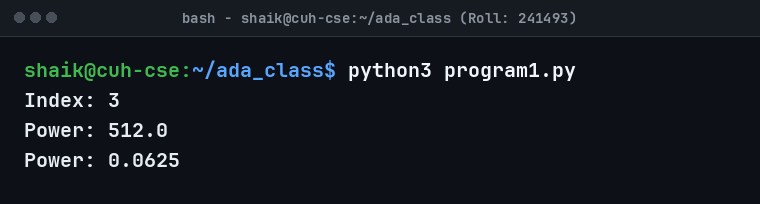
\includegraphics[width=0.88\textwidth]{Images/output_screenshot1.png}
\end{center}

\subsection*{GitHub Scan Code}
\begin{center}
    \begin{minipage}{0.3\textwidth}
        \centering
        % Generates a 2.5cm high QR code directly linking to the code file
        \qrcode[height=3.5cm]{https://github.com/gytdrop/ada_class/blob/main/program1.py} \\[0.2cm]
        \scriptsize\ttfamily Scan to view source code 
    \end{minipage}
\end{center}


% Add a horizontal line that indicates the END of the program.
\vspace{1cm}
\begin{center}
    \rule{1\textwidth}{1pt} % Clean, centered 1pt thick horizontal line
\end{center}
\pagebreak

% --- Program Section ---

\newprogram{Program 2}{Design a Sort class containing mergesort(arr: List[int]) -> List[int] and quicksort(arr:
List[int]) -> List[int] methods that accept an unsorted integer array and return the sorted
array.}

\subsection*{Code}
\begin{lstlisting}[language=Python]     % change the language attribute to C++ in case of C++ code.

from typing import List

class Sort:

    def merge_sort(self, arr: List[int]) -> List[int]:
        if len(arr) <= 1:
            return arr

        mid = len(arr) // 2

        left = self.merge_sort(arr[:mid])
        right = self.merge_sort(arr[mid:])

        return self.merge(left, right)

    def merge(self, left: List[int], right: List[int]) -> List[int]:
        result = []
        i = j = 0

        while i < len(left) and j < len(right):
            if left[i] <= right[j]:
                result.append(left[i])
                i += 1
            else:
                result.append(right[j])
                j += 1

        result.extend(left[i:])
        result.extend(right[j:])

        return result

    def quick_sort(self, arr: List[int]) -> List[int]:
        if len(arr) <= 1:
            return arr

        pivot = arr[len(arr) // 2]

        left = [x for x in arr if x < pivot]
        middle = [x for x in arr if x == pivot]
        right = [x for x in arr if x > pivot]

        return (
            self.quick_sort(left)
            + middle
            + self.quick_sort(right)
        )


# Example
s = Sort()

arr = [5, 2, 8, 1, 9, 3]

print("Merge Sort : " , s.merge_sort(arr))


print("Quick Sort : ", s.quick_sort(arr))

    
\end{lstlisting}

\subsection*{Output}
\begin{center}
    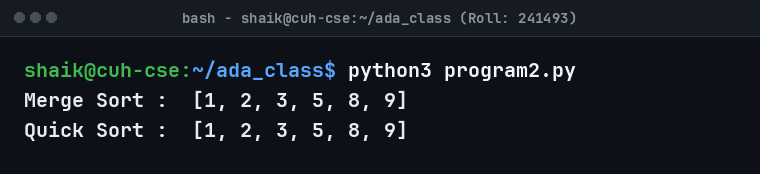
\includegraphics[width=0.88\textwidth]{Images/output_screenshot2.png}
\end{center}

\subsection*{GitHub Scan Code}
\begin{center}
    \begin{minipage}{0.3\textwidth}
        \centering
        % Generates a 2.5cm high QR code directly linking to the code file
        \qrcode[height=3.5cm]{https://github.com/gytdrop/ada_class/blob/main/program2.py} \\[0.2cm]
        \scriptsize\ttfamily Scan to view source code 
    \end{minipage}
\end{center}


% Add a horizontal line that indicates the END of the program.
\vspace{1cm}
\begin{center}
    \rule{1\textwidth}{1pt} % Clean, centered 1pt thick horizontal line
\end{center}
\pagebreak

% --- Program Section ---

\newprogram{Program 3}{Implement findKthLargest(nums: List[int], k: int) -> int and findMinMax(nums:
List[int]) -> Tuple[int, int] functions accepting an unsorted array, returning the -th element
and min-max pair.}

\subsection*{Code}
\begin{lstlisting}[language=Python]
from typing import List, Tuple

def findKthLargest(nums: List[int], k: int) -> int:
    nums.sort(reverse=True)
    return nums[k - 1]


def findMinMax(nums: List[int]) -> Tuple[int, int]:
    return min(nums), max(nums)


# Example
nums = [3, 1, 5, 2, 4]

print("Kth largest:", findKthLargest(nums, 2))
print("Min and Max:", findMinMax(nums))

\end{lstlisting}

\subsection*{Output}
\begin{center}
    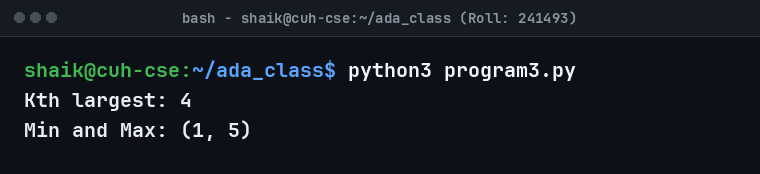
\includegraphics[width=0.88\textwidth]{Images/output_screenshot3.png}
\end{center}

\subsection*{GitHub Scan Code}
\begin{center}
    \begin{minipage}{0.3\textwidth}
        \centering
        % Generates a 2.5cm high QR code directly linking to the code file
        \qrcode[height=3.5cm]{https://github.com/gytdrop/ada_class/blob/main/program3.py} \\[0.2cm]
        \scriptsize\ttfamily Scan to view source code 
    \end{minipage}
\end{center}


% Add a horizontal line that indicates the END of the program.
\vspace{1cm}
\begin{center}
    \rule{1\textwidth}{1pt} % Clean, centered 1pt thick horizontal line
\end{center}
\pagebreak


% --- Program Section ---

\newprogram{Program 4}{Implement strassen-multiply(A: List[List[int]], B: List[List[int]]) ->
List[List[int]] accepting two matrices and returning their product matrix.}

\subsection*{Code}
\begin{lstlisting}[language=Python]
from typing import List

def strassen_multiply(A: List[List[int]], B: List[List[int]]) -> List[List[int]]:
    n = len(A)

    # Base case
    if n == 1:
        return [[A[0][0] * B[0][0]]]

    # Split matrices into 4 parts
    mid = n // 2

    A11 = [row[:mid] for row in A[:mid]]
    A12 = [row[mid:] for row in A[:mid]]
    A21 = [row[:mid] for row in A[mid:]]
    A22 = [row[mid:] for row in A[mid:]]

    B11 = [row[:mid] for row in B[:mid]]
    B12 = [row[mid:] for row in B[:mid]]
    B21 = [row[:mid] for row in B[mid:]]
    B22 = [row[mid:] for row in B[mid:]]

    def add(X, Y):
        return [[X[i][j] + Y[i][j] for j in range(len(X))]
                for i in range(len(X))]

    def subtract(X, Y):
        return [[X[i][j] - Y[i][j] for j in range(len(X))]
                for i in range(len(X))]

    # Strassen's 7 multiplications
    M1 = strassen_multiply(add(A11, A22), add(B11, B22))
    M2 = strassen_multiply(add(A21, A22), B11)
    M3 = strassen_multiply(A11, subtract(B12, B22))
    M4 = strassen_multiply(A22, subtract(B21, B11))
    M5 = strassen_multiply(add(A11, A12), B22)
    M6 = strassen_multiply(subtract(A21, A11), add(B11, B12))
    M7 = strassen_multiply(subtract(A12, A22), add(B21, B22))

    # Calculate result quadrants
    C11 = add(subtract(add(M1, M4), M5), M7)
    C12 = add(M3, M5)
    C21 = add(M2, M4)
    C22 = add(subtract(add(M1, M3), M2), M6)

    # Combine quadrants
    result = []

    for i in range(mid):
        result.append(C11[i] + C12[i])

    for i in range(mid):
        result.append(C21[i] + C22[i])

    return result


# Example
A = [
    [1, 2],
    [3, 4]
]

B = [
    [5, 6],
    [7, 8]
]

print(strassen_multiply(A, B))
\end{lstlisting}

\subsection*{Output}
\begin{center}
    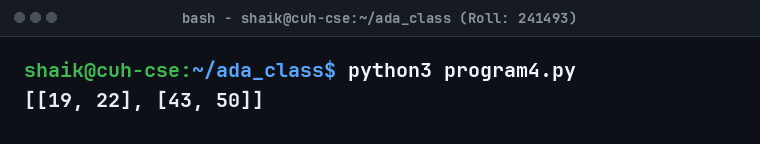
\includegraphics[width=0.88\textwidth]{Images/output_screenshot4.png}
\end{center}

\subsection*{GitHub Scan Code}
\begin{center}
    \begin{minipage}{0.3\textwidth}
        \centering
        % Generates a 2.5cm high QR code directly linking to the code file
        \qrcode[height=3.5cm]{https://github.com/gytdrop/ada_class/blob/main/program4.py} \\[0.2cm]
        \scriptsize\ttfamily Scan to view source code 
    \end{minipage}
\end{center}


% Add a horizontal line that indicates the END of the program.
\vspace{1cm}
\begin{center}
    \rule{1\textwidth}{1pt} % Clean, centered 1pt thick horizontal line
\end{center}
\pagebreak


% --- Program Section ---

\newprogram{Program 5}{Implement fractional-knapsack(weights: List[int], values: List[int], capacity: int)
-> float and job-scheduling(jobs: List[Job]) -> List[int] functions returning maximum
attainable profit and optimal job sequence.}

\subsection*{Code}
\begin{lstlisting}[language=Python]
from typing import List
from dataclasses import dataclass

@dataclass
class Job:
    id: int
    deadline: int
    profit: int

def fractional_knapsack(weights: List[int], values: List[int], capacity: int) -> float:
    # Calculate value/weight ratio
    items = [(values[i] / weights[i], weights[i], values[i])
             for i in range(len(weights))]

    # Sort by highest value/weight ratio
    items.sort(reverse=True)

    total_profit = 0.0

    for ratio, weight, value in items:
        if capacity == 0:
            break

        if weight <= capacity:
            total_profit += value
            capacity -= weight
        else:
            # Take only the fraction that fits
            total_profit += ratio * capacity
            capacity = 0

    return total_profit

def job_scheduling(jobs: List[Job]) -> List[int]:
    # Sort jobs by decreasing profit
    jobs.sort(key=lambda job: job.profit, reverse=True)

    max_deadline = max(job.deadline for job in jobs)

    # Time slots
    slots = [None] * (max_deadline + 1)

    # Schedule jobs
    for job in jobs:
        for slot in range(job.deadline, 0, -1):
            if slots[slot] is None:
                slots[slot] = job.id
                break

    # Return scheduled job IDs
    return [job_id for job_id in slots[1:] if job_id is not None]


# -----------------------------
# Fractional Knapsack Example
# -----------------------------

weights = [10, 20, 30]
values = [60, 100, 120]
capacity = 50

print("Maximum profit:",
      fractional_knapsack(weights, values, capacity))

# -----------------------------
# Job Scheduling Example
# -----------------------------

jobs = [
    Job(1, 2, 100),
    Job(2, 1, 19),
    Job(3, 2, 27),
    Job(4, 1, 25),
    Job(5, 3, 15)
]

print("Optimal job sequence:",
      job_scheduling(jobs))
\end{lstlisting}

\subsection*{Output}
\begin{center}
    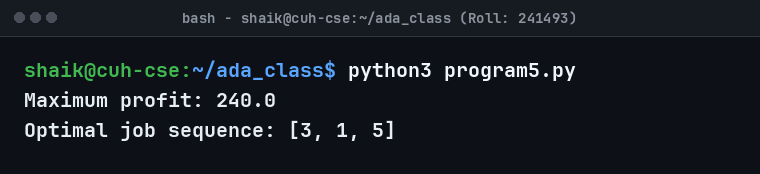
\includegraphics[width=0.88\textwidth]{Images/output_screenshot5.png}
\end{center}

\subsection*{GitHub Scan Code}
\begin{center}
    \begin{minipage}{0.3\textwidth}
        \centering
        % Generates a 2.5cm high QR code directly linking to the code file
        \qrcode[height=3.5cm]{https://github.com/gytdrop/ada_class/blob/main/program5.py} \\[0.2cm]
        \scriptsize\ttfamily Scan to view source code 
    \end{minipage}
\end{center}


% Add a horizontal line that indicates the END of the program.
\vspace{1cm}
\begin{center}
    \rule{1\textwidth}{1pt} % Clean, centered 1pt thick horizontal line
\end{center}
\pagebreak


% --- Program Section ---

\newprogram{Program 6}{Construct a Graph class with kruskal-mst() -> List[Edge] and prim-mst() -> List[Edge]
methods that process edge-weighted graph structures and return the MST edge set.}

\subsection*{Code}
\begin{lstlisting}[language=Python]
from dataclasses import dataclass
from typing import List
import heapq


@dataclass
class Edge:
    u: int
    v: int
    weight: int


class Graph:
    def __init__(self, vertices: int):
        self.vertices = vertices
        self.edges = []

    def add_edge(self, u: int, v: int, weight: int):
        self.edges.append(Edge(u, v, weight))

    # -------------------------
    # Kruskal's Algorithm
    # -------------------------
    def kruskal_mst(self) -> List[Edge]:
        parent = list(range(self.vertices))

        def find(x):
            if parent[x] != x:
                parent[x] = find(parent[x])
            return parent[x]

        def union(a, b):
            root_a = find(a)
            root_b = find(b)

            if root_a != root_b:
                parent[root_b] = root_a
                return True

            return False

        # Sort edges by weight
        edges = sorted(self.edges, key=lambda e: e.weight)

        mst = []

        for edge in edges:
            if union(edge.u, edge.v):
                mst.append(edge)

                if len(mst) == self.vertices - 1:
                    break

        return mst

    # -------------------------
    # Prim's Algorithm
    # -------------------------
    def prim_mst(self) -> List[Edge]:
        if self.vertices == 0:
            return []

        # Adjacency list
        graph = [[] for _ in range(self.vertices)]

        for edge in self.edges:
            graph[edge.u].append((edge.weight, edge.u, edge.v))
            graph[edge.v].append((edge.weight, edge.v, edge.u))

        visited = [False] * self.vertices
        heap = [(0, -1, 0)]

        mst = []

        while heap and len(mst) < self.vertices - 1:
            weight, parent, vertex = heapq.heappop(heap)

            if visited[vertex]:
                continue

            visited[vertex] = True

            if parent != -1:
                mst.append(Edge(parent, vertex, weight))

            for next_weight, u, v in graph[vertex]:
                if not visited[v]:
                    heapq.heappush(heap, (next_weight, vertex, v))

        return mst


# -------------------------
# Example
# -------------------------

g = Graph(4)

g.add_edge(0, 1, 10)
g.add_edge(0, 2, 6)
g.add_edge(0, 3, 5)
g.add_edge(1, 3, 15)
g.add_edge(2, 3, 4)

kruskal = g.kruskal_mst()
prim = g.prim_mst()

print("Kruskal MST:")
for edge in kruskal:
    print(edge.u, "-", edge.v, ":", edge.weight)

print("\nPrim MST:")
for edge in prim:
    print(edge.u, "-", edge.v, ":", edge.weight)
\end{lstlisting}

\subsection*{Output}
\begin{center}
    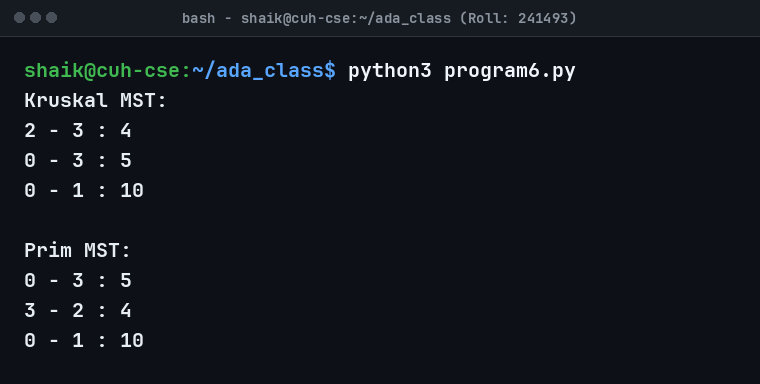
\includegraphics[width=0.88\textwidth]{Images/output_screenshot6.png}
\end{center}

\subsection*{GitHub Scan Code}
\begin{center}
    \begin{minipage}{0.3\textwidth}
        \centering
        % Generates a 2.5cm high QR code directly linking to the code file
        \qrcode[height=3.5cm]{https://github.com/gytdrop/ada_class/blob/main/program6.py} \\[0.2cm]
        \scriptsize\ttfamily Scan to view source code 
    \end{minipage}
\end{center}


% Add a horizontal line that indicates the END of the program.
\vspace{1cm}
\begin{center}
    \rule{1\textwidth}{1pt} % Clean, centered 1pt thick horizontal line
\end{center}
\pagebreak


% --- Program Section ---

\newprogram{Program 7}{Build a ShortestPath class containing dijkstra(src: int) -> List[int] and
bellman-ford(src: int) -> List[int] methods taking a starting node and returning distance
arrays (or error status for negative cycles).}

\subsection*{Code}


\begin{lstlisting}[language=python]
from typing import List
import heapq


class ShortestPath:
    def __init__(self, vertices: int):
        self.vertices = vertices
        self.edges = []

    def add_edge(self, u: int, v: int, weight: int):
        self.edges.append((u, v, weight))

    # -------------------------
    # Dijkstra's Algorithm
    # -------------------------
    def dijkstra(self, src: int) -> List[int]:
        graph = [[] for _ in range(self.vertices)]

        for u, v, weight in self.edges:
            graph[u].append((v, weight))

        distance = [float('inf')] * self.vertices
        distance[src] = 0

        pq = [(0, src)]

        while pq:
            dist, u = heapq.heappop(pq)

            if dist > distance[u]:
                continue

            for v, weight in graph[u]:
                new_dist = dist + weight

                if new_dist < distance[v]:
                    distance[v] = new_dist
                    heapq.heappush(pq, (new_dist, v))

        return distance
  
    # Bellman-Ford Algorithm
    def bellman_ford(self, src: int) -> List[int]:
        distance = [float('inf')] * self.vertices
        distance[src] = 0

        # Relax all edges V-1 times
        for _ in range(self.vertices - 1):
            changed = False

            for u, v, weight in self.edges:
                if distance[u] != float('inf') and \
                   distance[u] + weight < distance[v]:

                    distance[v] = distance[u] + weight
                    changed = True

            if not changed:
                break

        # Check for negative cycle
        for u, v, weight in self.edges:
            if distance[u] != float('inf') and \
               distance[u] + weight < distance[v]:
                return ["Negative cycle"]

        return distance


# Example
g = ShortestPath(5)
g.add_edge(0, 1, 4)
g.add_edge(0, 2, 1)
g.add_edge(2, 1, 2)
g.add_edge(1, 3, 1)
g.add_edge(2, 3, 5)
g.add_edge(3, 4, 3)

print("Dijkstra:", g.dijkstra(0))
print("Bellman-Ford:", g.bellman_ford(0))

\end{lstlisting}

\subsection*{Output}
\begin{center}
    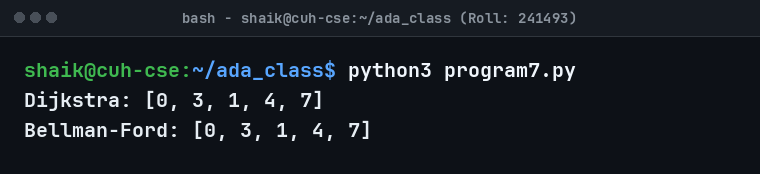
\includegraphics[width=0.88\textwidth]{Images/output_screenshot7.png}
\end{center}

\subsection*{GitHub Scan Code}
\begin{center}
    \begin{minipage}{0.3\textwidth}
        \centering
        % Generates a 2.5cm high QR code directly linking to the code file
        \qrcode[height=3.5cm]{https://github.com/gytdrop/ada_class/blob/main/program7.py} \\[0.2cm]
        \scriptsize\ttfamily Scan to view source code 
    \end{minipage}
\end{center}


% Add a horizontal line that indicates the END of the program.
\vspace{1cm}
\begin{center}
    \rule{1\textwidth}{1pt} % Clean, centered 1pt thick horizontal line
\end{center}
\pagebreak


% --- Program Section ---

\newprogram{Program 8}{Build a HuffmanCoder class with build-tree(frequencies: Dict[str, int]) -> Node and
generate-codes() -> Dict[str, str] methods accepting character frequencies and returning
binary encoding mappings.}

\subsection*{Code}


\begin{lstlisting}[language=python]

from typing import Dict
from dataclasses import dataclass
import heapq


@dataclass
class Node:
    char: str
    frequency: int
    left: object = None
    right: object = None


class HuffmanCoder:
    def __init__(self):
        self.root = None

    def build_tree(self, frequencies: Dict[str, int]) -> Node:
        heap = []
        count = 0

        # Create a node for every character
        for char, freq in frequencies.items():
            node = Node(char, freq)
            heapq.heappush(heap, (freq, count, node))
            count += 1

        # Combine two smallest nodes
        while len(heap) > 1:
            freq1, _, left = heapq.heappop(heap)
            freq2, _, right = heapq.heappop(heap)

            parent = Node("", freq1 + freq2, left, right)

            heapq.heappush(heap, (parent.frequency, count, parent))
            count += 1

        self.root = heap[0][2]
        return self.root

    def generate_codes(self) -> Dict[str, str]:
        codes = {}
        def generate(node, code):
            if node is None:
                return

            # Leaf node
            if node.left is None and node.right is None:
                codes[node.char] = code
                return

            generate(node.left, code + "0")
            generate(node.right, code + "1")

        generate(self.root, "")
        return codes
        
# Example
frequencies = {
    "A": 5,
    "B": 9,
    "C": 12,
    "D": 13,
    "E": 16,
    "F": 45
}
coder = HuffmanCoder()
coder.build_tree(frequencies)
codes = coder.generate_codes()
print("Huffman Codes:")
for char, code in codes.items():
    print(char, ":", code)
\end{lstlisting}

\subsection*{Output}
\begin{center}
    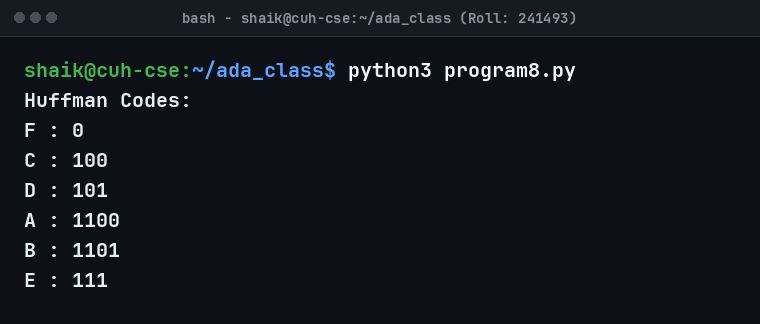
\includegraphics[width=0.88\textwidth]{Images/output_screenshot8.png}
\end{center}

\subsection*{GitHub Scan Code}
\begin{center}
    \begin{minipage}{0.3\textwidth}
        \centering
        % Generates a 2.5cm high QR code directly linking to the code file
        \qrcode[height=3.5cm]{https://github.com/gytdrop/ada_class/blob/main/program8.py} \\[0.2cm]
        \scriptsize\ttfamily Scan to view source code 
    \end{minipage}
\end{center}


% Add a horizontal line that indicates the END of the program.
\vspace{1cm}
\begin{center}
    \rule{1\textwidth}{1pt} % Clean, centered 1pt thick horizontal line
\end{center}
\pagebreak


% --- Program Section ---

\newprogram{Program 9}{Implement knapsack-01(weights: List[int], values: List[int], capacity: int) -> int
utilizing 2D/1D DP methods that accept item properties and return maximum value.}

\subsection*{Code}


\begin{lstlisting}[language=python]
from typing import List


# -------------------------
# 2D Dynamic Programming
# -------------------------
def knapsack_01_2d(
    weights: List[int],
    values: List[int],
    capacity: int
) -> int:

    n = len(weights)

    # dp[i][w] = maximum value using first i items
    # with capacity w
    dp = [[0] * (capacity + 1) for _ in range(n + 1)]

    for i in range(1, n + 1):
        weight = weights[i - 1]
        value = values[i - 1]

        for w in range(capacity + 1):

            # Don't take the item
            dp[i][w] = dp[i - 1][w]

            # Take the item if it fits
            if weight <= w:
                dp[i][w] = max(
                    dp[i][w],
                    value + dp[i - 1][w - weight]
                )

    return dp[n][capacity]

# -------------------------
# 1D Dynamic Programming
# -------------------------
def knapsack_01(
    weights: List[int],
    values: List[int],
    capacity: int
) -> int:

    dp = [0] * (capacity + 1)

    for i in range(len(weights)):
        weight = weights[i]
        value = values[i]

        # Traverse backwards so each item is used only once
        for w in range(capacity, weight - 1, -1):
            dp[w] = max(
                dp[w],
                value + dp[w - weight]
            )

    return dp[capacity]

# -------------------------
# Example
# -------------------------

weights = [1, 3, 4, 5]
values = [1, 4, 5, 7]
capacity = 7

print("2D DP:", knapsack_01_2d(weights, values, capacity))
print("1D DP:", knapsack_01(weights, values, capacity))

\end{lstlisting}

\subsection*{Output}
\begin{center}
    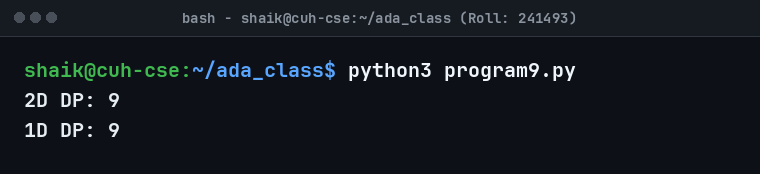
\includegraphics[width=0.88\textwidth]{Images/output_screenshot9.png}
\end{center}

\subsection*{GitHub Scan Code}
\begin{center}
    \begin{minipage}{0.3\textwidth}
        \centering
        % Generates a 2.5cm high QR code directly linking to the code file
        \qrcode[height=3.5cm]{https://github.com/gytdrop/ada_class/blob/main/program9.py} \\[0.2cm]
        \scriptsize\ttfamily Scan to view source code 
    \end{minipage}
\end{center}


% Add a horizontal line that indicates the END of the program.
\vspace{1cm}
\begin{center}
    \rule{1\textwidth}{1pt} % Clean, centered 1pt thick horizontal line
\end{center}
\pagebreak

% --- Program Section ---

\newprogram{Program 10}{Implement longestCommonSubsequence(text1: str, text2: str) -> int and
minDistance(word1: str, word2: str) -> int functions accepting input strings and returning
optimal length/edit operation counts.}

\subsection*{Code}


\begin{lstlisting}[language=python]
def longestCommonSubsequence(text1: str, text2: str) -> int:
    m = len(text1)
    n = len(text2)

    dp = [[0] * (n + 1) for _ in range(m + 1)]

    for i in range(1, m + 1):
        for j in range(1, n + 1):

            if text1[i - 1] == text2[j - 1]:
                dp[i][j] = 1 + dp[i - 1][j - 1]
            else:
                dp[i][j] = max(dp[i - 1][j], dp[i][j - 1])

    return dp[m][n]


def minDistance(word1: str, word2: str) -> int:
    m = len(word1)
    n = len(word2)

    dp = [[0] * (n + 1) for _ in range(m + 1)]

    # Converting empty string to word2
    for j in range(n + 1):
        dp[0][j] = j

    # Converting word1 to empty string
    for i in range(m + 1):
        dp[i][0] = i

    for i in range(1, m + 1):
        for j in range(1, n + 1):

            if word1[i - 1] == word2[j - 1]:
                dp[i][j] = dp[i - 1][j - 1]
            else:
                dp[i][j] = 1 + min(
                    dp[i - 1][j],      # Delete
                    dp[i][j - 1],      # Insert
                    dp[i - 1][j - 1]   # Replace
                )

    return dp[m][n]


# Examples

print(longestCommonSubsequence("abcde", "ace"))
print(minDistance("horse", "ros"))
\end{lstlisting}

\subsection*{Output}
\begin{center}
    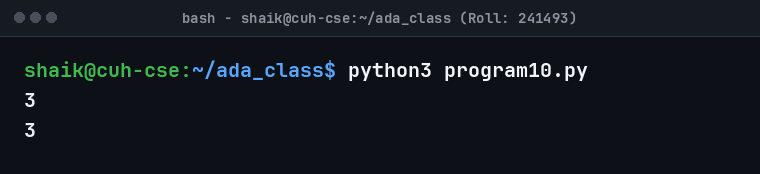
\includegraphics[width=0.88\textwidth]{Images/output_screenshot10.png}
\end{center}

\subsection*{GitHub Scan Code}
\begin{center}
    \begin{minipage}{0.3\textwidth}
        \centering
        % Generates a 2.5cm high QR code directly linking to the code file
        \qrcode[height=3.5cm]{https://github.com/gytdrop/ada_class/blob/main/program10.py} \\[0.2cm]
        \scriptsize\ttfamily Scan to view source code 
    \end{minipage}
\end{center}


% Add a horizontal line that indicates the END of the program.
\vspace{1cm}
\begin{center}
    \rule{1\textwidth}{1pt} % Clean, centered 1pt thick horizontal line
\end{center}
\pagebreak

% --- Program Section ---

\newprogram{Program 11}{Implement lengthOfLIS(nums: List[int]) -> int function accepting an integer array and
returning the length of the longest strictly increasing subsequence.}

\subsection*{Code}


\begin{lstlisting}[language=python]
from typing import List
import bisect

def lengthOfLIS(nums: List[int]) -> int:
    dp = []

    for num in nums:
        # Find the first element >= num
        pos = bisect.bisect_left(dp, num)

        if pos == len(dp):
            dp.append(num)
        else:
            dp[pos] = num

    return len(dp)


# Example
nums = [10, 9, 2, 5, 3, 7, 101, 18]

print("Length of LIS:", lengthOfLIS(nums))
\end{lstlisting}

\subsection*{Output}
\begin{center}
    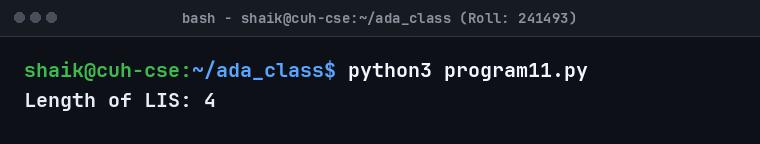
\includegraphics[width=0.88\textwidth]{Images/output_screenshot11.png}
\end{center}

\subsection*{GitHub Scan Code}
\begin{center}
    \begin{minipage}{0.3\textwidth}
        \centering
        % Generates a 2.5cm high QR code directly linking to the code file
        \qrcode[height=3.5cm]{https://github.com/gytdrop/ada_class/blob/main/program11.py} \\[0.2cm]
        \scriptsize\ttfamily Scan to view source code 
    \end{minipage}
\end{center}


% Add a horizontal line that indicates the END of the program.
\vspace{1cm}
\begin{center}
    \rule{1\textwidth}{1pt} % Clean, centered 1pt thick horizontal line
\end{center}
\pagebreak

% --- Program Section ---

\newprogram{Program 12}{Implement floyd-warshall(graph: List[List[int]]) -> List[List[int]] and
optimal-bst(keys: List[int], freq: List[int]) -> int accepting distance/frequency
matrices and returning shortest path or cost matrices.}

\subsection*{Code}


\begin{lstlisting}[language=python]
from typing import List


def floyd_warshall(graph: List[List[int]]) -> List[List[int]]:
    n = len(graph)

    # Make a copy so the original graph is not modified
    dist = [row[:] for row in graph]

    for k in range(n):
        for i in range(n):
            for j in range(n):
                if dist[i][k] != float('inf') and dist[k][j] != float('inf'):
                    dist[i][j] = min(
                        dist[i][j],
                        dist[i][k] + dist[k][j]
                    )

    return dist


def optimal_bst(keys: List[int], freq: List[int]) -> int:
    n = len(keys)

    if n == 0:
        return 0

    # dp[i][j] = minimum cost for keys i through j
    dp = [[0] * n for _ in range(n)]
    # Prefix sum for frequencies
    prefix = [0] * (n + 1)
    for i in range(n):
        prefix[i + 1] = prefix[i] + freq[i]
    def total_freq(i, j):
        return prefix[j + 1] - prefix[i]
    # One-key trees
    for i in range(n):
        dp[i][i] = freq[i]
    # Consider increasing lengths
    for length in range(2, n + 1):
        for i in range(n - length + 1):
            j = i + length - 1
            dp[i][j] = float('inf')
            # Try every key as root
            for root in range(i, j + 1):
                left = dp[i][root - 1] if root > i else 0
                right = dp[root + 1][j] if root < j else 0
                cost = left + right + total_freq(i, j)
                dp[i][j] = min(dp[i][j], cost)
    return dp[0][n - 1]

# Floyd-Warshall Example
INF = float('inf')
graph = [
    [0, 3, INF, 7],
    [8, 0, 2, INF],
    [5, INF, 0, 1],
    [2, INF, INF, 0]
]
result = floyd_warshall(graph)
print("Shortest path matrix:")
for row in result:
    print(row)
# Optimal BST Example
keys = [10, 12, 20]
freq = [34, 8, 50]

print("\nOptimal BST cost:", optimal_bst(keys, freq))
\end{lstlisting}

\subsection*{Output}
\begin{center}
    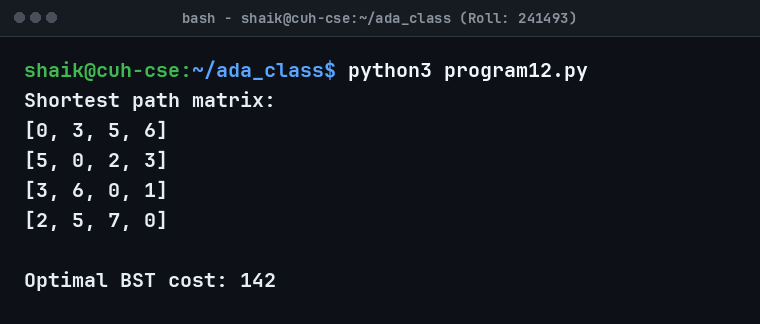
\includegraphics[width=0.88\textwidth]{Images/output_screenshot12.png}
\end{center}

\subsection*{GitHub Scan Code}
\begin{center}
    \begin{minipage}{0.3\textwidth}
        \centering
        % Generates a 2.5cm high QR code directly linking to the code file
        \qrcode[height=3.5cm]{https://github.com/gytdrop/ada_class/blob/main/program12.py} \\[0.2cm]
        \scriptsize\ttfamily Scan to view source code 
    \end{minipage}
\end{center}


% Add a horizontal line that indicates the END of the program.
\vspace{1cm}
\begin{center}
    \rule{1\textwidth}{1pt} % Clean, centered 1pt thick horizontal line
\end{center}
\pagebreak

% --- Program Section ---

\newprogram{Program 13}{Create a TSPSolver class with solve-tsp(dist-matrix: List[List[int]]) -> int taking an
adjacency matrix and returning the minimum tour cost.}

\subsection*{Code}


\begin{lstlisting}[language=python]
from typing import List


class TSPSolver:

    def solve_tsp(self, dist_matrix: List[List[int]]) -> int:
        n = len(dist_matrix)

        if n == 0:
            return 0

        # dp[mask][i] = minimum cost to visit all cities
        # in mask and end at city i
        dp = [[float('inf')] * n for _ in range(1 << n)]

        # Start from city 0
        dp[1][0] = 0

        for mask in range(1 << n):
            for current in range(n):

                if dp[mask][current] == float('inf'):
                    continue

                # Try visiting every unvisited city
                for next_city in range(n):

                    if mask & (1 << next_city):
                        continue

                    new_mask = mask | (1 << next_city)

                    new_cost = (
                        dp[mask][current]
                        + dist_matrix[current][next_city]
                    )

                    dp[new_mask][next_city] = min(
                        dp[new_mask][next_city],
                        new_cost
                    )

        # All cities visited
        full_mask = (1 << n) - 1

        # Return to starting city
        answer = float('inf')

        for city in range(1, n):
            answer = min(
                answer,
                dp[full_mask][city] + dist_matrix[city][0]
            )

        return answer


# -------------------------
# Example
# -------------------------

dist_matrix = [
    [0, 10, 15, 20],
    [10, 0, 35, 25],
    [15, 35, 0, 30],
    [20, 25, 30, 0]
]

solver = TSPSolver()

print("Minimum tour cost:",
      solver.solve_tsp(dist_matrix))
\end{lstlisting}

\subsection*{Output}
\begin{center}
    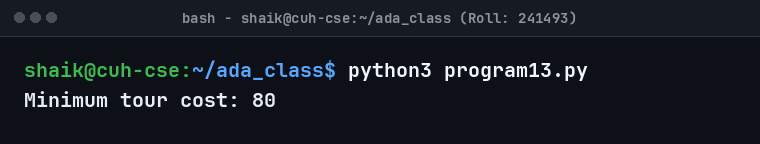
\includegraphics[width=0.88\textwidth]{Images/output_screenshot13.png}
\end{center}

\subsection*{GitHub Scan Code}
\begin{center}
    \begin{minipage}{0.3\textwidth}
        \centering
        % Generates a 2.5cm high QR code directly linking to the code file
        \qrcode[height=3.5cm]{https://github.com/gytdrop/ada_class/blob/main/program13.py} \\[0.2cm]
        \scriptsize\ttfamily Scan to view source code 
    \end{minipage}
\end{center}


% Add a horizontal line that indicates the END of the program.
\vspace{1cm}
\begin{center}
    \rule{1\textwidth}{1pt} % Clean, centered 1pt thick horizontal line
\end{center}
\pagebreak

% --- Program Section ---

\newprogram{Program 14}{Implement solveNQueens(n: int) -> List[List[str]] function taking board dimension and
returning all valid board layout configurations. }
\subsection*{Code}


\begin{lstlisting}[language=python]
from typing import List


def solveNQueens(n: int) -> List[List[str]]:
    result = []

    board = [["."] * n for _ in range(n)]

    columns = set()
    diagonals = set()
    anti_diagonals = set()

    def backtrack(row):
        # All queens placed
        if row == n:
            result.append(["".join(row) for row in board])
            return

        for col in range(n):

            # Check if column or diagonal is already occupied
            if col in columns:
                continue

            if row - col in diagonals:
                continue

            if row + col in anti_diagonals:
                continue

            # Place queen
            board[row][col] = "Q"
            columns.add(col)
            diagonals.add(row - col)
            anti_diagonals.add(row + col)

            # Move to next row
            backtrack(row + 1)

            # Remove queen (backtrack)
            board[row][col] = "."
            columns.remove(col)
            diagonals.remove(row - col)
            anti_diagonals.remove(row + col)

    backtrack(0)

    return result


# Example
n = 4

solutions = solveNQueens(n)

print("Number of solutions:", len(solutions))

for solution in solutions:
    for row in solution:
        print(row)
    print()
\end{lstlisting}

\subsection*{Output}
\begin{center}
    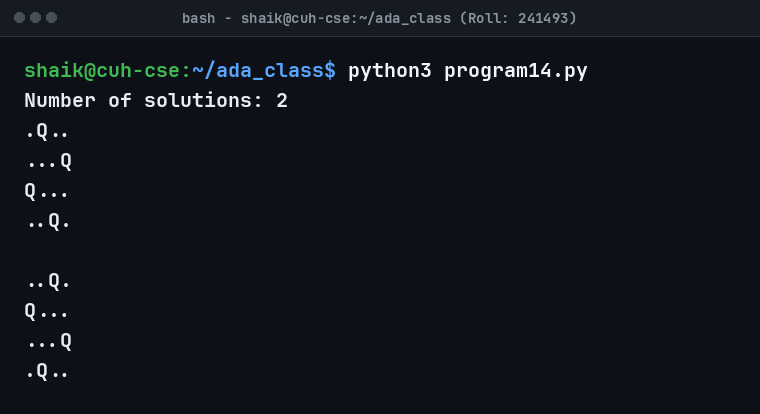
\includegraphics[width=0.88\textwidth]{Images/output_screenshot14.png}
\end{center}

\subsection*{GitHub Scan Code}
\begin{center}
    \begin{minipage}{0.3\textwidth}
        \centering
        % Generates a 2.5cm high QR code directly linking to the code file
        \qrcode[height=3.5cm]{https://github.com/gytdrop/ada_class/blob/main/program14.py} \\[0.2cm]
        \scriptsize\ttfamily Scan to view source code 
    \end{minipage}
\end{center}


% Add a horizontal line that indicates the END of the program.
\vspace{1cm}
\begin{center}
    \rule{1\textwidth}{1pt} % Clean, centered 1pt thick horizontal line
\end{center}
\pagebreak

% --- Program Section ---

\newprogram{Program 15}{ Build a GraphBacktracker class featuring graph-coloring(m: int) -> List[int] and
hamiltonian-cycle() -> List[int] methods returning vertex-color mappings and valid path
cycles.}
\subsection*{Code}


\begin{lstlisting}[language=python]
from typing import List


class GraphBacktracker:

    def __init__(self, graph: List[List[int]]):
        self.graph = graph
        self.n = len(graph)

    # --------------------------------
    # Graph Coloring
    # --------------------------------
    def graph_coloring(self, m: int) -> List[int]:
        colors = [0] * self.n

        def is_safe(vertex, color):
            for neighbor in range(self.n):
                if self.graph[vertex][neighbor] and colors[neighbor] == color:
                    return False
            return True

        def backtrack(vertex):
            if vertex == self.n:
                return True

            for color in range(1, m + 1):
                if is_safe(vertex, color):
                    colors[vertex] = color

                    if backtrack(vertex + 1):
                        return True

                    colors[vertex] = 0

            return False

        if backtrack(0):
            return colors

        return []


    # --------------------------------
    # Hamiltonian Cycle
    # --------------------------------
    def hamiltonian_cycle(self) -> List[int]:
        if self.n == 0:
            return []

        path = [-1] * self.n
        path[0] = 0

        def is_safe(vertex, position):
            # Must be connected to previous vertex
            if not self.graph[path[position - 1]][vertex]:
                return False

            # Vertex must not already be in path
            if vertex in path:
                return False

            return True

        def backtrack(position):
            if position == self.n:
                # Last vertex must connect to first vertex
                return self.graph[path[-1]][path[0]] != 0

            for vertex in range(1, self.n):
                if is_safe(vertex, position):
                    path[position] = vertex

                    if backtrack(position + 1):
                        return True

                    path[position] = -1

            return False

        if backtrack(1):
            # Add starting vertex to show complete cycle
            return path + [path[0]]

        return []


# --------------------------------
# Example Graph
# --------------------------------

graph = [
    [0, 1, 1, 1],
    [1, 0, 1, 1],
    [1, 1, 0, 1],
    [1, 1, 1, 0]
]

solver = GraphBacktracker(graph)


# Graph Coloring
print("Graph Coloring:")
print(solver.graph_coloring(3))


# Hamiltonian Cycle
print("\nHamiltonian Cycle:")
print(solver.hamiltonian_cycle())
\end{lstlisting}

\subsection*{Output}
\begin{center}
    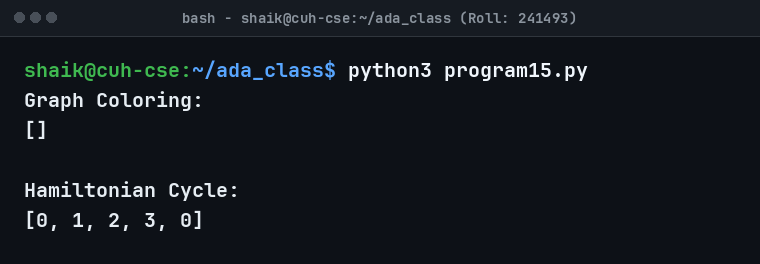
\includegraphics[width=0.88\textwidth]{Images/output_screenshot15.png}
\end{center}

\subsection*{GitHub Scan Code}
\begin{center}
    \begin{minipage}{0.3\textwidth}
        \centering
        % Generates a 2.5cm high QR code directly linking to the code file
        \qrcode[height=3.5cm]{https://github.com/gytdrop/ada_class/blob/main/program15.py} \\[0.2cm]
        \scriptsize\ttfamily Scan to view source code 
    \end{minipage}
\end{center}


% Add a horizontal line that indicates the END of the program.
\vspace{1cm}
\begin{center}
    \rule{1\textwidth}{1pt} % Clean, centered 1pt thick horizontal line
\end{center}
\pagebreak

% --- Program Section ---

\newprogram{Program 16}{ Implement strStr(haystack: str, needle: str) -> int using KMP and a Randomizer class with
getRandom() -> int for stream sampling, accepting text/pattern strings or stream data and returning
indices or sampled elements.}
\subsection*{Code}


\begin{lstlisting}[language=python]
from typing import Iterator, Optional
import random

# KMP String Matching
def strStr(haystack: str, needle: str) -> int:
    if needle == "":
        return 0

    # Build LPS (Longest Prefix Suffix) array
    lps = [0] * len(needle)

    length = 0
    i = 1

    while i < len(needle):
        if needle[i] == needle[length]:
            length += 1
            lps[i] = length
            i += 1
        elif length > 0:
            length = lps[length - 1]
        else:
            lps[i] = 0
            i += 1

    # Search needle inside haystack
    i = 0
    j = 0

    while i < len(haystack):
        if haystack[i] == needle[j]:
            i += 1
            j += 1

            if j == len(needle):
                return i - j

        elif j > 0:
            j = lps[j - 1]
        else:
            i += 1

    return -1
# Reservoir Sampling
class Randomizer:

    def __init__(self, stream):
        self.stream = stream
        self.selected = None

    def getRandom(self) -> int:
        """
        Return one uniformly random element from the stream.
        """

        selected = None

        for i, value in enumerate(self.stream, start=1):

            # Replace selected element with probability 1/i
            if random.randint(1, i) == 1:
                selected = value

        return selected
# Examples
print("KMP result:")
print(strStr("hello", "ll"))

print("\nRandom stream sample:")

stream = [10, 20, 30, 40, 50]

randomizer = Randomizer(stream)

print(randomizer.getRandom())
\end{lstlisting}

\subsection*{Output}
\begin{center}
    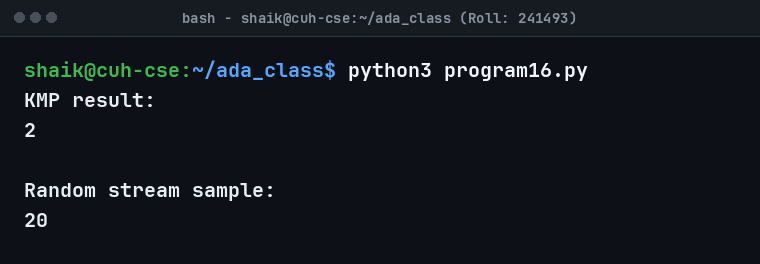
\includegraphics[width=0.88\textwidth]{Images/output_screenshot16.png}
\end{center}

\subsection*{GitHub Scan Code}
\begin{center}
    \begin{minipage}{0.3\textwidth}
        \centering
        % Generates a 2.5cm high QR code directly linking to the code file
        \qrcode[height=3.5cm]{https://github.com/gytdrop/ada_class/blob/main/program16.py} \\[0.2cm]
        \scriptsize\ttfamily Scan to view source code 
    \end{minipage}
\end{center}


% Add a horizontal line that indicates the END of the program.
\vspace{1cm}
\begin{center}
    \rule{1\textwidth}{1pt} % Clean, centered 1pt thick horizontal line
\end{center}
\pagebreak



% ==================== END OF DOCUMENT ====================
% --- Global Lab Repository Link Placeholder ---
\subsection*{Lab Work Repository}
\begin{center}
    \begin{minipage}{0.4\textwidth}
        \centering
        % Generates a QR code linking to the master folder repository
        \qrcode[height=3.5cm]{https://github.com/gytdrop/ada_class} \\[0.2cm]
        \small\bfseries Scan for Complete Lab Folder [cite: 49]
    \end{minipage}
\end{center}

\end{document}
